\documentclass[1p]{elsarticle_modified}
%\bibliographystyle{elsarticle-num}

%\usepackage[colorlinks]{hyperref}
%\usepackage{abbrmath_seonhwa} %\Abb, \Ascr, \Acal ,\Abf, \Afrak
\usepackage{amsfonts}
\usepackage{amssymb}
\usepackage{amsmath}
\usepackage{amsthm}
\usepackage{scalefnt}
\usepackage{amsbsy}
\usepackage{kotex}
\usepackage{caption}
\usepackage{subfig}
\usepackage{color}
\usepackage{graphicx}
\usepackage{xcolor} %% white, black, red, green, blue, cyan, magenta, yellow
\usepackage{float}
\usepackage{setspace}
\usepackage{hyperref}

\usepackage{tikz}
\usetikzlibrary{arrows}

\usepackage{multirow}
\usepackage{array} % fixed length table
\usepackage{hhline}

%%%%%%%%%%%%%%%%%%%%%
\makeatletter
\renewcommand*\env@matrix[1][\arraystretch]{%
	\edef\arraystretch{#1}%
	\hskip -\arraycolsep
	\let\@ifnextchar\new@ifnextchar
	\array{*\c@MaxMatrixCols c}}
\makeatother %https://tex.stackexchange.com/questions/14071/how-can-i-increase-the-line-spacing-in-a-matrix
%%%%%%%%%%%%%%%

\usepackage[normalem]{ulem}

\newcommand{\msout}[1]{\ifmmode\text{\sout{\ensuremath{#1}}}\else\sout{#1}\fi}
%SOURCE: \msout is \stkout macro in https://tex.stackexchange.com/questions/20609/strikeout-in-math-mode

\newcommand{\cancel}[1]{
	\ifmmode
	{\color{red}\msout{#1}}
	\else
	{\color{red}\sout{#1}}
	\fi
}

\newcommand{\add}[1]{
	{\color{blue}\uwave{#1}}
}

\newcommand{\replace}[2]{
	\ifmmode
	{\color{red}\msout{#1}}{\color{blue}\uwave{#2}}
	\else
	{\color{red}\sout{#1}}{\color{blue}\uwave{#2}}
	\fi
}

\newcommand{\Sol}{\mathcal{S}} %segment
\newcommand{\D}{D} %diagram
\newcommand{\A}{\mathcal{A}} %arc


%%%%%%%%%%%%%%%%%%%%%%%%%%%%%5 test

\def\sl{\operatorname{\textup{SL}}(2,\Cbb)}
\def\psl{\operatorname{\textup{PSL}}(2,\Cbb)}
\def\quan{\mkern 1mu \triangleright \mkern 1mu}

\theoremstyle{definition}
\newtheorem{thm}{Theorem}[section]
\newtheorem{prop}[thm]{Proposition}
\newtheorem{lem}[thm]{Lemma}
\newtheorem{ques}[thm]{Question}
\newtheorem{cor}[thm]{Corollary}
\newtheorem{defn}[thm]{Definition}
\newtheorem{exam}[thm]{Example}
\newtheorem{rmk}[thm]{Remark}
\newtheorem{alg}[thm]{Algorithm}

\newcommand{\I}{\sqrt{-1}}
\begin{document}

%\begin{frontmatter}
%
%\title{Boundary parabolic representations of knots up to 8 crossings}
%
%%% Group authors per affiliation:
%\author{Yunhi Cho} 
%\address{Department of Mathematics, University of Seoul, Seoul, Korea}
%\ead{yhcho@uos.ac.kr}
%
%
%\author{Seonhwa Kim} %\fnref{s_kim}}
%\address{Center for Geometry and Physics, Institute for Basic Science, Pohang, 37673, Korea}
%\ead{ryeona17@ibs.re.kr}
%
%\author{Hyuk Kim}
%\address{Department of Mathematical Sciences, Seoul National University, Seoul 08826, Korea}
%\ead{hyukkim@snu.ac.kr}
%
%\author{Seokbeom Yoon}
%\address{Department of Mathematical Sciences, Seoul National University, Seoul, 08826,  Korea}
%\ead{sbyoon15@snu.ac.kr}
%
%\begin{abstract}
%We find all boundary parabolic representation of knots up to 8 crossings.
%
%\end{abstract}
%\begin{keyword}
%    \MSC[2010] 57M25 
%\end{keyword}
%
%\end{frontmatter}

%\linenumbers
%\tableofcontents
%
\newcommand\colored[1]{\textcolor{white}{\rule[-0.35ex]{0.8em}{1.4ex}}\kern-0.8em\color{red} #1}%
%\newcommand\colored[1]{\textcolor{white}{ #1}\kern-2.17ex	\textcolor{white}{ #1}\kern-1.81ex	\textcolor{white}{ #1}\kern-2.15ex\color{red}#1	}

{\Large $\underline{11a_{155}~(K11a_{155})}$}

\setlength{\tabcolsep}{10pt}
\renewcommand{\arraystretch}{1.6}
\vspace{1cm}\begin{tabular}{m{100pt}>{\centering\arraybackslash}m{274pt}}
\multirow{5}{120pt}{
	\centering
	\includegraphics[width=112pt]{../../../GIT/diagram.site/Diagrams/png/404_11a_155.png}\\
\ \ \ A knot diagram\footnotemark}&
\allowdisplaybreaks
\textbf{Linearized knot diagam} \\
\cline{2-2}
 &
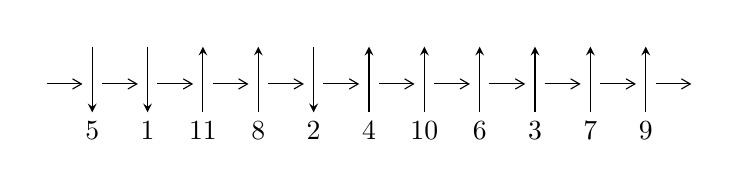
\begin{tikzpicture}[x=20pt, y=17pt]
	% nodes
	\node (C0) at (0, 0) {};
	\node (C1) at (1, 0) {};
	\node (C1U) at (1, +1) {};
	\node (C1D) at (1, -1) {5};

	\node (C2) at (2, 0) {};
	\node (C2U) at (2, +1) {};
	\node (C2D) at (2, -1) {1};

	\node (C3) at (3, 0) {};
	\node (C3U) at (3, +1) {};
	\node (C3D) at (3, -1) {11};

	\node (C4) at (4, 0) {};
	\node (C4U) at (4, +1) {};
	\node (C4D) at (4, -1) {8};

	\node (C5) at (5, 0) {};
	\node (C5U) at (5, +1) {};
	\node (C5D) at (5, -1) {2};

	\node (C6) at (6, 0) {};
	\node (C6U) at (6, +1) {};
	\node (C6D) at (6, -1) {4};

	\node (C7) at (7, 0) {};
	\node (C7U) at (7, +1) {};
	\node (C7D) at (7, -1) {10};

	\node (C8) at (8, 0) {};
	\node (C8U) at (8, +1) {};
	\node (C8D) at (8, -1) {6};

	\node (C9) at (9, 0) {};
	\node (C9U) at (9, +1) {};
	\node (C9D) at (9, -1) {3};

	\node (C10) at (10, 0) {};
	\node (C10U) at (10, +1) {};
	\node (C10D) at (10, -1) {7};

	\node (C11) at (11, 0) {};
	\node (C11U) at (11, +1) {};
	\node (C11D) at (11, -1) {9};
	\node (C12) at (12, 0) {};

	% arrows
	\draw[->,>={angle 60}]
	(C0) edge (C1) (C1) edge (C2) (C2) edge (C3) (C3) edge (C4) (C4) edge (C5) (C5) edge (C6) (C6) edge (C7) (C7) edge (C8) (C8) edge (C9) (C9) edge (C10) (C10) edge (C11) (C11) edge (C12) ;	\draw[->,>=stealth]
	(C1U) edge (C1D) (C2U) edge (C2D) (C3D) edge (C3U) (C4D) edge (C4U) (C5U) edge (C5D) (C6D) edge (C6U) (C7D) edge (C7U) (C8D) edge (C8U) (C9D) edge (C9U) (C10D) edge (C10U) (C11D) edge (C11U) ;
	\end{tikzpicture} \\
\hhline{~~} \\& 
\textbf{Solving Sequence} \\ \cline{2-2} 
 &
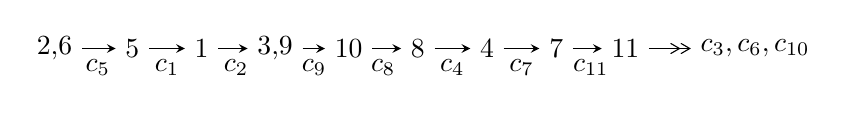
\begin{tikzpicture}[x=25pt, y=7pt]
	% node
	\node (A0) at (-1/8, 0) {2,6};
	\node (A1) at (1, 0) {5};
	\node (A2) at (2, 0) {1};
	\node (A3) at (49/16, 0) {3,9};
	\node (A4) at (33/8, 0) {10};
	\node (A5) at (41/8, 0) {8};
	\node (A6) at (49/8, 0) {4};
	\node (A7) at (57/8, 0) {7};
	\node (A8) at (65/8, 0) {11};
	\node (C1) at (1/2, -1) {$c_{5}$};
	\node (C2) at (3/2, -1) {$c_{1}$};
	\node (C3) at (5/2, -1) {$c_{2}$};
	\node (C4) at (29/8, -1) {$c_{9}$};
	\node (C5) at (37/8, -1) {$c_{8}$};
	\node (C6) at (45/8, -1) {$c_{4}$};
	\node (C7) at (53/8, -1) {$c_{7}$};
	\node (C8) at (61/8, -1) {$c_{11}$};
	\node (A9) at (10, 0) {$c_{3},c_{6},c_{10}$};

	% edge
	\draw[->,>=stealth]	
	(A0) edge (A1) (A1) edge (A2) (A2) edge (A3) (A3) edge (A4) (A4) edge (A5) (A5) edge (A6) (A6) edge (A7) (A7) edge (A8) ;
	\draw[->>,>={angle 60}]	
	(A8) edge (A9);
\end{tikzpicture} \\ 

\end{tabular} \\

\footnotetext{
The image of knot diagram is generated by the software ``\textbf{Draw programme}" developed by Andrew Bartholomew(\url{http://www.layer8.co.uk/maths/draw/index.htm\#Running-draw}), where we modified some parts for our purpose(\url{https://github.com/CATsTAILs/LinksPainter}).
}\phantom \\ \newline 
\centering \textbf{Ideals for irreducible components\footnotemark of $X_{\text{par}}$} 
 
\begin{align*}
I^u_{1}&=\langle 
634617868812 u^{44}+5120393538096 u^{43}+\cdots+30290494853 b-88597448899,\\
\phantom{I^u_{1}}&\phantom{= \langle  }19298245499249 u^{44}+173772806942140 u^{43}+\cdots+302904948530 a-151790191623698,\\
\phantom{I^u_{1}}&\phantom{= \langle  }u^{45}+10 u^{44}+\cdots-62 u-10\rangle \\
I^u_{2}&=\langle 
9 u^{29}-22 u^{28}+\cdots+2 b+15,\;-15 u^{29} a+21 u^{29}+\cdots-25 a+47,\;u^{30}-3 u^{29}+\cdots+6 u-1\rangle \\
I^u_{3}&=\langle 
-10 u^{15}+19 u^{14}+\cdots+b+11,\;-33 u^{15}+77 u^{14}+\cdots+2 a+60,\\
\phantom{I^u_{3}}&\phantom{= \langle  }u^{16}-3 u^{15}+u^{14}+8 u^{13}-11 u^{12}-3 u^{11}+16 u^{10}-5 u^9-12 u^8+4 u^7+18 u^6-18 u^5- u^4+9 u^3- u^2-4 u+2\rangle \\
I^u_{4}&=\langle 
b+a+1,\;a^2+2 a+2,\;u+1\rangle \\
I^u_{5}&=\langle 
b^2+1,\;a-1,\;u+1\rangle \\
\\
\end{align*}
\raggedright * 5 irreducible components of $\dim_{\mathbb{C}}=0$, with total 125 representations.\\
\footnotetext{All coefficients of polynomials are rational numbers. But the coefficients are sometimes approximated in decimal forms when there is not enough margin.}
\newpage
\renewcommand{\arraystretch}{1}
\centering \section*{I. $I^u_{1}= \langle 6.35\times10^{11} u^{44}+5.12\times10^{12} u^{43}+\cdots+3.03\times10^{10} b-8.86\times10^{10},\;1.93\times10^{13} u^{44}+1.74\times10^{14} u^{43}+\cdots+3.03\times10^{11} a-1.52\times10^{14},\;u^{45}+10 u^{44}+\cdots-62 u-10 \rangle$}
\flushleft \textbf{(i) Arc colorings}\\
\begin{tabular}{m{7pt} m{180pt} m{7pt} m{180pt} }
\flushright $a_{2}=$&$\begin{pmatrix}0\\u\end{pmatrix}$ \\
\flushright $a_{6}=$&$\begin{pmatrix}1\\0\end{pmatrix}$ \\
\flushright $a_{5}=$&$\begin{pmatrix}1\\- u^2\end{pmatrix}$ \\
\flushright $a_{1}=$&$\begin{pmatrix}u\\- u^3+u\end{pmatrix}$ \\
\flushright $a_{3}=$&$\begin{pmatrix}- u^3\\u^5- u^3+u\end{pmatrix}$ \\
\flushright $a_{9}=$&$\begin{pmatrix}-63.7106 u^{44}-573.688 u^{43}+\cdots+2769.67 u+501.115\\-20.9511 u^{44}-169.043 u^{43}+\cdots+154.125 u+2.92493\end{pmatrix}$ \\
\flushright $a_{10}=$&$\begin{pmatrix}-27.4817 u^{44}-253.810 u^{43}+\cdots+1512.06 u+294.306\\-21.4161 u^{44}-184.268 u^{43}+\cdots+590.907 u+90.3501\end{pmatrix}$ \\
\flushright $a_{8}=$&$\begin{pmatrix}-42.7595 u^{44}-404.645 u^{43}+\cdots+2615.55 u+498.190\\-20.9511 u^{44}-169.043 u^{43}+\cdots+154.125 u+2.92493\end{pmatrix}$ \\
\flushright $a_{4}=$&$\begin{pmatrix}-0.151903 u^{44}+14.1733 u^{43}+\cdots-560.112 u-114.459\\21.5585 u^{44}+195.648 u^{43}+\cdots-991.029 u-171.620\end{pmatrix}$ \\
\flushright $a_{7}=$&$\begin{pmatrix}-31.1941 u^{44}-298.498 u^{43}+\cdots+2176.62 u+428.069\\-6.32145 u^{44}-47.9083 u^{43}+\cdots-67.2357 u-22.6589\end{pmatrix}$ \\
\flushright $a_{11}=$&$\begin{pmatrix}32.4369 u^{44}+282.562 u^{43}+\cdots-863.523 u-114.918\\4.19050 u^{44}+26.6301 u^{43}+\cdots+372.503 u+93.7023\end{pmatrix}$\\ \flushright $a_{11}=$&$\begin{pmatrix}32.4369 u^{44}+282.562 u^{43}+\cdots-863.523 u-114.918\\4.19050 u^{44}+26.6301 u^{43}+\cdots+372.503 u+93.7023\end{pmatrix}$\\&\end{tabular}
\flushleft \textbf{(ii) Obstruction class $= -1$}\\~\\
\flushleft \textbf{(iii) Cusp Shapes $= \frac{3963758068051}{30290494853} u^{44}+\frac{32549076872033}{30290494853} u^{43}+\cdots-\frac{27811268065342}{30290494853} u+\frac{968878849396}{30290494853}$}\\~\\
\newpage\renewcommand{\arraystretch}{1}
\flushleft \textbf{(iv) u-Polynomials at the component}\newline \\
\begin{tabular}{m{50pt}|m{274pt}}
Crossings & \hspace{64pt}u-Polynomials at each crossing \\
\hline $$\begin{aligned}c_{1},c_{5}\end{aligned}$$&$\begin{aligned}
&u^{45}+10 u^{44}+\cdots-62 u-10
\end{aligned}$\\
\hline $$\begin{aligned}c_{2}\end{aligned}$$&$\begin{aligned}
&u^{45}+18 u^{44}+\cdots+1884 u+100
\end{aligned}$\\
\hline $$\begin{aligned}c_{3},c_{6}\end{aligned}$$&$\begin{aligned}
&u^{45}+3 u^{44}+\cdots+6 u-1
\end{aligned}$\\
\hline $$\begin{aligned}c_{4},c_{9}\end{aligned}$$&$\begin{aligned}
&u^{45}- u^{44}+\cdots+8 u-1
\end{aligned}$\\
\hline $$\begin{aligned}c_{7},c_{10}\end{aligned}$$&$\begin{aligned}
&u^{45}+11 u^{44}+\cdots-398 u-26
\end{aligned}$\\
\hline $$\begin{aligned}c_{8},c_{11}\end{aligned}$$&$\begin{aligned}
&u^{45}+2 u^{44}+\cdots-3 u-2
\end{aligned}$\\
\hline
\end{tabular}\\~\\
\newpage\renewcommand{\arraystretch}{1}
\flushleft \textbf{(v) Riley Polynomials at the component}\newline \\
\begin{tabular}{m{50pt}|m{274pt}}
Crossings & \hspace{64pt}Riley Polynomials at each crossing \\
\hline $$\begin{aligned}c_{1},c_{5}\end{aligned}$$&$\begin{aligned}
&y^{45}-18 y^{44}+\cdots+1884 y-100
\end{aligned}$\\
\hline $$\begin{aligned}c_{2}\end{aligned}$$&$\begin{aligned}
&y^{45}+18 y^{44}+\cdots+438256 y-10000
\end{aligned}$\\
\hline $$\begin{aligned}c_{3},c_{6}\end{aligned}$$&$\begin{aligned}
&y^{45}+33 y^{44}+\cdots-36 y-1
\end{aligned}$\\
\hline $$\begin{aligned}c_{4},c_{9}\end{aligned}$$&$\begin{aligned}
&y^{45}-7 y^{44}+\cdots+20 y-1
\end{aligned}$\\
\hline $$\begin{aligned}c_{7},c_{10}\end{aligned}$$&$\begin{aligned}
&y^{45}+23 y^{44}+\cdots+14052 y-676
\end{aligned}$\\
\hline $$\begin{aligned}c_{8},c_{11}\end{aligned}$$&$\begin{aligned}
&y^{45}+14 y^{44}+\cdots-123 y-4
\end{aligned}$\\
\hline
\end{tabular}\\~\\
\newpage\flushleft \textbf{(vi) Complex Volumes and Cusp Shapes}
$$\begin{array}{c|c|c}  
\text{Solutions to }I^u_{1}& \I (\text{vol} + \sqrt{-1}CS) & \text{Cusp shape}\\
 \hline 
\begin{aligned}
u &= -0.901122 + 0.391026 I \\
a &= -2.22398 - 0.09634 I \\
b &= -0.507989 - 0.720972 I\end{aligned}
 & -4.13007 + 2.02494 I & \phantom{-0.000000 } 0. - 5.73901 I \\ \hline\begin{aligned}
u &= -0.901122 - 0.391026 I \\
a &= -2.22398 + 0.09634 I \\
b &= -0.507989 + 0.720972 I\end{aligned}
 & -4.13007 - 2.02494 I & \phantom{-0.000000 -}0. + 5.73901 I \\ \hline\begin{aligned}
u &= -0.576298 + 0.870424 I \\
a &= -0.93549 + 1.15916 I \\
b &= -1.09116 + 1.03701 I\end{aligned}
 & \phantom{-}2.66346 - 6.40405 I & \phantom{-}5.00000 + 4.59149 I \\ \hline\begin{aligned}
u &= -0.576298 - 0.870424 I \\
a &= -0.93549 - 1.15916 I \\
b &= -1.09116 - 1.03701 I\end{aligned}
 & \phantom{-}2.66346 + 6.40405 I & \phantom{-}5.00000 - 4.59149 I \\ \hline\begin{aligned}
u &= -0.848723 + 0.610214 I \\
a &= -2.00602 + 1.35310 I \\
b &= -1.58039 - 0.17618 I\end{aligned}
 & \phantom{-}3.17854 + 2.40398 I & \phantom{-}17.2523 - 3.9170 I \\ \hline\begin{aligned}
u &= -0.848723 - 0.610214 I \\
a &= -2.00602 - 1.35310 I \\
b &= -1.58039 + 0.17618 I\end{aligned}
 & \phantom{-}3.17854 - 2.40398 I & \phantom{-}17.2523 + 3.9170 I \\ \hline\begin{aligned}
u &= \phantom{-}0.801098 + 0.511169 I \\
a &= -0.632677 - 0.499625 I \\
b &= \phantom{-}0.08297 + 1.43190 I\end{aligned}
 & -2.91066 - 1.58558 I & \phantom{-}0.87322 + 3.50523 I \\ \hline\begin{aligned}
u &= \phantom{-}0.801098 - 0.511169 I \\
a &= -0.632677 + 0.499625 I \\
b &= \phantom{-}0.08297 - 1.43190 I\end{aligned}
 & -2.91066 + 1.58558 I & \phantom{-}0.87322 - 3.50523 I \\ \hline\begin{aligned}
u &= \phantom{-}0.913441 + 0.533170 I \\
a &= \phantom{-}0.586441 + 0.383102 I \\
b &= -0.28087 - 1.44457 I\end{aligned}
 & -3.30005 - 2.64955 I & \phantom{-0.000000 } 0 \\ \hline\begin{aligned}
u &= \phantom{-}0.913441 - 0.533170 I \\
a &= \phantom{-}0.586441 - 0.383102 I \\
b &= -0.28087 + 1.44457 I\end{aligned}
 & -3.30005 + 2.64955 I & \phantom{-0.000000 } 0\\
 \hline 
 \end{array}$$\newpage$$\begin{array}{c|c|c}  
\text{Solutions to }I^u_{1}& \I (\text{vol} + \sqrt{-1}CS) & \text{Cusp shape}\\
 \hline 
\begin{aligned}
u &= -0.523749 + 0.936187 I \\
a &= \phantom{-}0.920068 - 0.987167 I \\
b &= \phantom{-}1.07979 - 1.07052 I\end{aligned}
 & -0.63452 - 12.54830 I & \phantom{-}5.00000 + 6.69848 I \\ \hline\begin{aligned}
u &= -0.523749 - 0.936187 I \\
a &= \phantom{-}0.920068 + 0.987167 I \\
b &= \phantom{-}1.07979 + 1.07052 I\end{aligned}
 & -0.63452 + 12.54830 I & \phantom{-}5.00000 - 6.69848 I \\ \hline\begin{aligned}
u &= -0.238075 + 0.894367 I \\
a &= -0.175446 - 0.518756 I \\
b &= -0.415208 - 0.426850 I\end{aligned}
 & \phantom{-}1.09089 + 2.34622 I & \phantom{-}6.24165 - 8.56728 I \\ \hline\begin{aligned}
u &= -0.238075 - 0.894367 I \\
a &= -0.175446 + 0.518756 I \\
b &= -0.415208 + 0.426850 I\end{aligned}
 & \phantom{-}1.09089 - 2.34622 I & \phantom{-}6.24165 + 8.56728 I \\ \hline\begin{aligned}
u &= -0.960767 + 0.492160 I \\
a &= \phantom{-}1.083620 - 0.193384 I \\
b &= \phantom{-}0.391029 + 0.437334 I\end{aligned}
 & -1.62646 + 1.74137 I & \phantom{-0.000000 } 0 \\ \hline\begin{aligned}
u &= -0.960767 - 0.492160 I \\
a &= \phantom{-}1.083620 + 0.193384 I \\
b &= \phantom{-}0.391029 - 0.437334 I\end{aligned}
 & -1.62646 - 1.74137 I & \phantom{-0.000000 } 0 \\ \hline\begin{aligned}
u &= \phantom{-}1.086040 + 0.097856 I \\
a &= -0.337473 - 0.512143 I \\
b &= \phantom{-}0.602346 + 1.260120 I\end{aligned}
 & -8.25548 + 0.14518 I & -5.86924 + 0. I\phantom{ +0.000000I} \\ \hline\begin{aligned}
u &= \phantom{-}1.086040 - 0.097856 I \\
a &= -0.337473 + 0.512143 I \\
b &= \phantom{-}0.602346 - 1.260120 I\end{aligned}
 & -8.25548 - 0.14518 I & -5.86924 + 0. I\phantom{ +0.000000I} \\ \hline\begin{aligned}
u &= \phantom{-}0.675748 + 0.600812 I \\
a &= \phantom{-}0.487260 + 0.009850 I \\
b &= -0.361960 - 0.696002 I\end{aligned}
 & \phantom{-}1.72135 + 0.10542 I & \phantom{-}9.89084 - 0.57623 I \\ \hline\begin{aligned}
u &= \phantom{-}0.675748 - 0.600812 I \\
a &= \phantom{-}0.487260 - 0.009850 I \\
b &= -0.361960 + 0.696002 I\end{aligned}
 & \phantom{-}1.72135 - 0.10542 I & \phantom{-}9.89084 + 0.57623 I\\
 \hline 
 \end{array}$$\newpage$$\begin{array}{c|c|c}  
\text{Solutions to }I^u_{1}& \I (\text{vol} + \sqrt{-1}CS) & \text{Cusp shape}\\
 \hline 
\begin{aligned}
u &= \phantom{-}0.960223 + 0.625182 I \\
a &= -0.287488 - 0.184192 I \\
b &= \phantom{-}0.092459 + 0.799602 I\end{aligned}
 & \phantom{-}0.86875 - 4.99777 I & \phantom{-0.000000 } 0 \\ \hline\begin{aligned}
u &= \phantom{-}0.960223 - 0.625182 I \\
a &= -0.287488 + 0.184192 I \\
b &= \phantom{-}0.092459 - 0.799602 I\end{aligned}
 & \phantom{-}0.86875 + 4.99777 I & \phantom{-0.000000 } 0 \\ \hline\begin{aligned}
u &= \phantom{-}1.155300 + 0.090732 I \\
a &= \phantom{-}0.136153 - 0.470997 I \\
b &= -0.479381 + 1.128020 I\end{aligned}
 & -3.98808 - 5.11963 I & \phantom{-0.000000 } 0 \\ \hline\begin{aligned}
u &= \phantom{-}1.155300 - 0.090732 I \\
a &= \phantom{-}0.136153 + 0.470997 I \\
b &= -0.479381 - 1.128020 I\end{aligned}
 & -3.98808 + 5.11963 I & \phantom{-0.000000 } 0 \\ \hline\begin{aligned}
u &= -0.503146 + 0.661088 I \\
a &= \phantom{-}1.36514 - 1.24377 I \\
b &= \phantom{-}0.943060 - 0.848825 I\end{aligned}
 & -3.52213 - 1.72391 I & \phantom{-}1.61111 + 1.48880 I \\ \hline\begin{aligned}
u &= -0.503146 - 0.661088 I \\
a &= \phantom{-}1.36514 + 1.24377 I \\
b &= \phantom{-}0.943060 + 0.848825 I\end{aligned}
 & -3.52213 + 1.72391 I & \phantom{-}1.61111 - 1.48880 I \\ \hline\begin{aligned}
u &= -0.464268 + 1.091500 I \\
a &= \phantom{-}0.334880 + 0.281474 I \\
b &= \phantom{-}0.504214 + 0.379227 I\end{aligned}
 & -1.04118 + 7.01442 I & \phantom{-0.000000 } 0 \\ \hline\begin{aligned}
u &= -0.464268 - 1.091500 I \\
a &= \phantom{-}0.334880 - 0.281474 I \\
b &= \phantom{-}0.504214 - 0.379227 I\end{aligned}
 & -1.04118 - 7.01442 I & \phantom{-0.000000 } 0 \\ \hline\begin{aligned}
u &= -0.887945 + 0.799772 I \\
a &= \phantom{-}0.877042 + 0.320791 I \\
b &= \phantom{-}0.449189 + 0.781343 I\end{aligned}
 & -1.90231 + 0.74732 I & \phantom{-0.000000 } 0 \\ \hline\begin{aligned}
u &= -0.887945 - 0.799772 I \\
a &= \phantom{-}0.877042 - 0.320791 I \\
b &= \phantom{-}0.449189 - 0.781343 I\end{aligned}
 & -1.90231 - 0.74732 I & \phantom{-0.000000 } 0\\
 \hline 
 \end{array}$$\newpage$$\begin{array}{c|c|c}  
\text{Solutions to }I^u_{1}& \I (\text{vol} + \sqrt{-1}CS) & \text{Cusp shape}\\
 \hline 
\begin{aligned}
u &= -1.036610 + 0.611989 I \\
a &= \phantom{-}2.03296 - 0.73494 I \\
b &= \phantom{-}1.16696 + 1.08790 I\end{aligned}
 & -5.03326 + 6.70507 I & \phantom{-0.000000 } 0 \\ \hline\begin{aligned}
u &= -1.036610 - 0.611989 I \\
a &= \phantom{-}2.03296 + 0.73494 I \\
b &= \phantom{-}1.16696 - 1.08790 I\end{aligned}
 & -5.03326 - 6.70507 I & \phantom{-0.000000 } 0 \\ \hline\begin{aligned}
u &= -1.077580 + 0.695430 I \\
a &= -1.83741 + 0.52861 I \\
b &= -1.15966 - 1.26459 I\end{aligned}
 & \phantom{-}1.13119 + 12.21450 I & \phantom{-0.000000 } 0 \\ \hline\begin{aligned}
u &= -1.077580 - 0.695430 I \\
a &= -1.83741 - 0.52861 I \\
b &= -1.15966 + 1.26459 I\end{aligned}
 & \phantom{-}1.13119 - 12.21450 I & \phantom{-0.000000 } 0 \\ \hline\begin{aligned}
u &= \phantom{-}1.283260 + 0.065802 I \\
a &= -0.167563 + 0.367408 I \\
b &= \phantom{-}0.576462 - 1.035600 I\end{aligned}
 & -7.63721 - 10.29470 I & \phantom{-0.000000 } 0 \\ \hline\begin{aligned}
u &= \phantom{-}1.283260 - 0.065802 I \\
a &= -0.167563 - 0.367408 I \\
b &= \phantom{-}0.576462 + 1.035600 I\end{aligned}
 & -7.63721 + 10.29470 I & \phantom{-0.000000 } 0 \\ \hline\begin{aligned}
u &= -1.121770 + 0.698957 I \\
a &= \phantom{-}1.70890 - 0.60391 I \\
b &= \phantom{-}1.12635 + 1.27279 I\end{aligned}
 & -2.4765 + 18.5384 I & \phantom{-0.000000 } 0 \\ \hline\begin{aligned}
u &= -1.121770 - 0.698957 I \\
a &= \phantom{-}1.70890 + 0.60391 I \\
b &= \phantom{-}1.12635 - 1.27279 I\end{aligned}
 & -2.4765 - 18.5384 I & \phantom{-0.000000 } 0 \\ \hline\begin{aligned}
u &= -1.046500 + 0.828865 I \\
a &= -0.567749 - 0.408140 I \\
b &= \phantom{-}0.007330 - 0.774890 I\end{aligned}
 & -2.28132 + 5.64431 I & \phantom{-0.000000 } 0 \\ \hline\begin{aligned}
u &= -1.046500 - 0.828865 I \\
a &= -0.567749 + 0.408140 I \\
b &= \phantom{-}0.007330 + 0.774890 I\end{aligned}
 & -2.28132 - 5.64431 I & \phantom{-0.000000 } 0\\
 \hline 
 \end{array}$$\newpage$$\begin{array}{c|c|c}  
\text{Solutions to }I^u_{1}& \I (\text{vol} + \sqrt{-1}CS) & \text{Cusp shape}\\
 \hline 
\begin{aligned}
u &= -1.317060 + 0.458673 I \\
a &= -0.374157 + 0.197877 I \\
b &= -0.070789 - 0.321439 I\end{aligned}
 & -4.37062 - 0.52471 I & \phantom{-0.000000 } 0 \\ \hline\begin{aligned}
u &= -1.317060 - 0.458673 I \\
a &= -0.374157 - 0.197877 I \\
b &= -0.070789 + 0.321439 I\end{aligned}
 & -4.37062 + 0.52471 I & \phantom{-0.000000 } 0 \\ \hline\begin{aligned}
u &= -0.554028 + 0.236204 I \\
a &= \phantom{-}1.09200 + 1.81024 I \\
b &= \phantom{-}0.284535 + 0.576144 I\end{aligned}
 & -3.33768 + 0.83512 I & \phantom{-}2.33619 - 3.83248 I \\ \hline\begin{aligned}
u &= -0.554028 - 0.236204 I \\
a &= \phantom{-}1.09200 - 1.81024 I \\
b &= \phantom{-}0.284535 - 0.576144 I\end{aligned}
 & -3.33768 - 0.83512 I & \phantom{-}2.33619 + 3.83248 I \\ \hline\begin{aligned}
u &= \phantom{-}0.365045\phantom{ +0.000000I} \\
a &= \phantom{-}1.44199\phantom{ +0.000000I} \\
b &= -0.718548\phantom{ +0.000000I}\end{aligned}
 & \phantom{-}1.11526\phantom{ +0.000000I} & \phantom{-}5.80750\phantom{ +0.000000I}\\
 \hline 
 \end{array}$$\newpage\newpage\renewcommand{\arraystretch}{1}
\centering \section*{II. $I^u_{2}= \langle 9 u^{29}-22 u^{28}+\cdots+2 b+15,\;-15 u^{29} a+21 u^{29}+\cdots-25 a+47,\;u^{30}-3 u^{29}+\cdots+6 u-1 \rangle$}
\flushleft \textbf{(i) Arc colorings}\\
\begin{tabular}{m{7pt} m{180pt} m{7pt} m{180pt} }
\flushright $a_{2}=$&$\begin{pmatrix}0\\u\end{pmatrix}$ \\
\flushright $a_{6}=$&$\begin{pmatrix}1\\0\end{pmatrix}$ \\
\flushright $a_{5}=$&$\begin{pmatrix}1\\- u^2\end{pmatrix}$ \\
\flushright $a_{1}=$&$\begin{pmatrix}u\\- u^3+u\end{pmatrix}$ \\
\flushright $a_{3}=$&$\begin{pmatrix}- u^3\\u^5- u^3+u\end{pmatrix}$ \\
\flushright $a_{9}=$&$\begin{pmatrix}a\\-\frac{9}{2} u^{29}+11 u^{28}+\cdots+\frac{65}{2} u-\frac{15}{2}\end{pmatrix}$ \\
\flushright $a_{10}=$&$\begin{pmatrix}-\frac{1}{2} u^{29}+u^{28}+\cdots+a-\frac{1}{2}\\-5 u^{29}+11 u^{28}+\cdots+31 u-7\end{pmatrix}$ \\
\flushright $a_{8}=$&$\begin{pmatrix}\frac{9}{2} u^{29}-11 u^{28}+\cdots+a+\frac{15}{2}\\-\frac{9}{2} u^{29}+11 u^{28}+\cdots+\frac{65}{2} u-\frac{15}{2}\end{pmatrix}$ \\
\flushright $a_{4}=$&$\begin{pmatrix}3 u^{29} a-\frac{1}{2} u^{29}+\cdots+5 a-\frac{13}{2}\\-\frac{5}{2} u^{29} a+6 u^{28} a+\cdots-\frac{7}{2} a+1\end{pmatrix}$ \\
\flushright $a_{7}=$&$\begin{pmatrix}- u^{29} a+\frac{11}{2} u^{29}+\cdots-\frac{67}{2} u+\frac{15}{2}\\\frac{1}{2} u^{29} a-\frac{1}{2} u^{29}+\cdots+\frac{1}{2} a+\frac{1}{2}\end{pmatrix}$ \\
\flushright $a_{11}=$&$\begin{pmatrix}-\frac{9}{2} u^{29} a+5 u^{29}+\cdots-\frac{15}{2} a+8\\1\end{pmatrix}$\\ \flushright $a_{11}=$&$\begin{pmatrix}-\frac{9}{2} u^{29} a+5 u^{29}+\cdots-\frac{15}{2} a+8\\1\end{pmatrix}$\\&\end{tabular}
\flushleft \textbf{(ii) Obstruction class $= -1$}\\~\\
\flushleft \textbf{(iii) Cusp Shapes $= 25 u^{29}-52 u^{28}-102 u^{27}+385 u^{26}+29 u^{25}-1217 u^{24}+842 u^{23}+2204 u^{22}-3082 u^{21}-2095 u^{20}+6222 u^{19}-293 u^{18}-8211 u^{17}+4523 u^{16}+7118 u^{15}-8008 u^{14}-3146 u^{13}+8424 u^{12}-1074 u^{11}-5710 u^{10}+3096 u^9+2146 u^8-2516 u^7+20 u^6+1054 u^5-509 u^4-102 u^3+231 u^2-129 u+29$}\\~\\
\newpage\renewcommand{\arraystretch}{1}
\flushleft \textbf{(iv) u-Polynomials at the component}\newline \\
\begin{tabular}{m{50pt}|m{274pt}}
Crossings & \hspace{64pt}u-Polynomials at each crossing \\
\hline $$\begin{aligned}c_{1},c_{5}\end{aligned}$$&$\begin{aligned}
&(u^{30}-3 u^{29}+\cdots+6 u-1)^{2}
\end{aligned}$\\
\hline $$\begin{aligned}c_{2}\end{aligned}$$&$\begin{aligned}
&(u^{30}+13 u^{29}+\cdots+8 u+1)^{2}
\end{aligned}$\\
\hline $$\begin{aligned}c_{3},c_{6}\end{aligned}$$&$\begin{aligned}
&u^{60}+7 u^{59}+\cdots+2 u^2+2
\end{aligned}$\\
\hline $$\begin{aligned}c_{4},c_{9}\end{aligned}$$&$\begin{aligned}
&u^{60}- u^{59}+\cdots+64 u+94
\end{aligned}$\\
\hline $$\begin{aligned}c_{7},c_{10}\end{aligned}$$&$\begin{aligned}
&(u^{30}-9 u^{29}+\cdots-14 u+1)^{2}
\end{aligned}$\\
\hline $$\begin{aligned}c_{8},c_{11}\end{aligned}$$&$\begin{aligned}
&u^{60}+9 u^{59}+\cdots+16 u+1
\end{aligned}$\\
\hline
\end{tabular}\\~\\
\newpage\renewcommand{\arraystretch}{1}
\flushleft \textbf{(v) Riley Polynomials at the component}\newline \\
\begin{tabular}{m{50pt}|m{274pt}}
Crossings & \hspace{64pt}Riley Polynomials at each crossing \\
\hline $$\begin{aligned}c_{1},c_{5}\end{aligned}$$&$\begin{aligned}
&(y^{30}-13 y^{29}+\cdots-8 y+1)^{2}
\end{aligned}$\\
\hline $$\begin{aligned}c_{2}\end{aligned}$$&$\begin{aligned}
&(y^{30}+11 y^{29}+\cdots-52 y+1)^{2}
\end{aligned}$\\
\hline $$\begin{aligned}c_{3},c_{6}\end{aligned}$$&$\begin{aligned}
&y^{60}-7 y^{59}+\cdots+8 y+4
\end{aligned}$\\
\hline $$\begin{aligned}c_{4},c_{9}\end{aligned}$$&$\begin{aligned}
&y^{60}+y^{59}+\cdots-322944 y+8836
\end{aligned}$\\
\hline $$\begin{aligned}c_{7},c_{10}\end{aligned}$$&$\begin{aligned}
&(y^{30}+19 y^{29}+\cdots-76 y+1)^{2}
\end{aligned}$\\
\hline $$\begin{aligned}c_{8},c_{11}\end{aligned}$$&$\begin{aligned}
&y^{60}-21 y^{59}+\cdots+26 y+1
\end{aligned}$\\
\hline
\end{tabular}\\~\\
\newpage\flushleft \textbf{(vi) Complex Volumes and Cusp Shapes}
$$\begin{array}{c|c|c}  
\text{Solutions to }I^u_{2}& \I (\text{vol} + \sqrt{-1}CS) & \text{Cusp shape}\\
 \hline 
\begin{aligned}
u &= \phantom{-}0.465809 + 0.917860 I \\
a &= -0.989163 - 0.559689 I \\
b &= -1.128460 - 0.357199 I\end{aligned}
 & \phantom{-}2.56109 + 3.64354 I & \phantom{-}6.72804 - 6.05682 I \\ \hline\begin{aligned}
u &= \phantom{-}0.465809 + 0.917860 I \\
a &= \phantom{-}0.752661 + 0.348017 I \\
b &= \phantom{-}0.715413 + 0.742706 I\end{aligned}
 & \phantom{-}2.56109 + 3.64354 I & \phantom{-}6.72804 - 6.05682 I \\ \hline\begin{aligned}
u &= \phantom{-}0.465809 - 0.917860 I \\
a &= -0.989163 + 0.559689 I \\
b &= -1.128460 + 0.357199 I\end{aligned}
 & \phantom{-}2.56109 - 3.64354 I & \phantom{-}6.72804 + 6.05682 I \\ \hline\begin{aligned}
u &= \phantom{-}0.465809 - 0.917860 I \\
a &= \phantom{-}0.752661 - 0.348017 I \\
b &= \phantom{-}0.715413 - 0.742706 I\end{aligned}
 & \phantom{-}2.56109 - 3.64354 I & \phantom{-}6.72804 + 6.05682 I \\ \hline\begin{aligned}
u &= \phantom{-}0.558834 + 0.876988 I \\
a &= \phantom{-}0.968989 + 0.487384 I \\
b &= \phantom{-}0.838815 + 0.150681 I\end{aligned}
 & \phantom{-}3.22316 + 0.83801 I & \phantom{-}8.60335 + 3.08812 I \\ \hline\begin{aligned}
u &= \phantom{-}0.558834 + 0.876988 I \\
a &= -0.669745 - 0.519770 I \\
b &= -0.929490 - 0.703123 I\end{aligned}
 & \phantom{-}3.22316 + 0.83801 I & \phantom{-}8.60335 + 3.08812 I \\ \hline\begin{aligned}
u &= \phantom{-}0.558834 - 0.876988 I \\
a &= \phantom{-}0.968989 - 0.487384 I \\
b &= \phantom{-}0.838815 - 0.150681 I\end{aligned}
 & \phantom{-}3.22316 - 0.83801 I & \phantom{-}8.60335 - 3.08812 I \\ \hline\begin{aligned}
u &= \phantom{-}0.558834 - 0.876988 I \\
a &= -0.669745 + 0.519770 I \\
b &= -0.929490 + 0.703123 I\end{aligned}
 & \phantom{-}3.22316 - 0.83801 I & \phantom{-}8.60335 - 3.08812 I \\ \hline\begin{aligned}
u &= -0.847173 + 0.604187 I \\
a &= -1.63142 + 1.20812 I \\
b &= -1.55381 + 0.24780 I\end{aligned}
 & \phantom{-}3.14397 + 2.38497 I & \phantom{-}13.36478 - 4.30077 I \\ \hline\begin{aligned}
u &= -0.847173 + 0.604187 I \\
a &= -2.00619 + 1.33601 I \\
b &= -1.312340 - 0.515721 I\end{aligned}
 & \phantom{-}3.14397 + 2.38497 I & \phantom{-}13.36478 - 4.30077 I\\
 \hline 
 \end{array}$$\newpage$$\begin{array}{c|c|c}  
\text{Solutions to }I^u_{2}& \I (\text{vol} + \sqrt{-1}CS) & \text{Cusp shape}\\
 \hline 
\begin{aligned}
u &= -0.847173 - 0.604187 I \\
a &= -1.63142 - 1.20812 I \\
b &= -1.55381 - 0.24780 I\end{aligned}
 & \phantom{-}3.14397 - 2.38497 I & \phantom{-}13.36478 + 4.30077 I \\ \hline\begin{aligned}
u &= -0.847173 - 0.604187 I \\
a &= -2.00619 - 1.33601 I \\
b &= -1.312340 + 0.515721 I\end{aligned}
 & \phantom{-}3.14397 - 2.38497 I & \phantom{-}13.36478 + 4.30077 I \\ \hline\begin{aligned}
u &= -0.745543 + 0.602909 I \\
a &= \phantom{-}1.51667 - 0.00542 I \\
b &= \phantom{-}0.884770 - 0.652787 I\end{aligned}
 & -0.67785 - 3.97386 I & \phantom{-}7.94279 + 4.15081 I \\ \hline\begin{aligned}
u &= -0.745543 + 0.602909 I \\
a &= \phantom{-}2.27309 - 0.86759 I \\
b &= \phantom{-}1.47023 + 1.29190 I\end{aligned}
 & -0.67785 - 3.97386 I & \phantom{-}7.94279 + 4.15081 I \\ \hline\begin{aligned}
u &= -0.745543 - 0.602909 I \\
a &= \phantom{-}1.51667 + 0.00542 I \\
b &= \phantom{-}0.884770 + 0.652787 I\end{aligned}
 & -0.67785 + 3.97386 I & \phantom{-}7.94279 - 4.15081 I \\ \hline\begin{aligned}
u &= -0.745543 - 0.602909 I \\
a &= \phantom{-}2.27309 + 0.86759 I \\
b &= \phantom{-}1.47023 - 1.29190 I\end{aligned}
 & -0.67785 + 3.97386 I & \phantom{-}7.94279 - 4.15081 I \\ \hline\begin{aligned}
u &= \phantom{-}0.713795 + 0.638334 I \\
a &= \phantom{-}0.029316 - 1.007750 I \\
b &= -0.94994 - 1.09157 I\end{aligned}
 & \phantom{-}1.88688 + 0.24232 I & \phantom{-}9.09491 - 2.16089 I \\ \hline\begin{aligned}
u &= \phantom{-}0.713795 + 0.638334 I \\
a &= \phantom{-}0.835125 + 0.889030 I \\
b &= \phantom{-}0.060739 - 0.151129 I\end{aligned}
 & \phantom{-}1.88688 + 0.24232 I & \phantom{-}9.09491 - 2.16089 I \\ \hline\begin{aligned}
u &= \phantom{-}0.713795 - 0.638334 I \\
a &= \phantom{-}0.029316 + 1.007750 I \\
b &= -0.94994 + 1.09157 I\end{aligned}
 & \phantom{-}1.88688 - 0.24232 I & \phantom{-}9.09491 + 2.16089 I \\ \hline\begin{aligned}
u &= \phantom{-}0.713795 - 0.638334 I \\
a &= \phantom{-}0.835125 - 0.889030 I \\
b &= \phantom{-}0.060739 + 0.151129 I\end{aligned}
 & \phantom{-}1.88688 - 0.24232 I & \phantom{-}9.09491 + 2.16089 I\\
 \hline 
 \end{array}$$\newpage$$\begin{array}{c|c|c}  
\text{Solutions to }I^u_{2}& \I (\text{vol} + \sqrt{-1}CS) & \text{Cusp shape}\\
 \hline 
\begin{aligned}
u &= -1.08167\phantom{ +0.000000I} \\
a &= \phantom{-}0.611909 + 0.400488 I \\
b &= -0.054055 - 0.901769 I\end{aligned}
 & -3.22581\phantom{ +0.000000I} & \phantom{-}2.05120\phantom{ +0.000000I} \\ \hline\begin{aligned}
u &= -1.08167\phantom{ +0.000000I} \\
a &= \phantom{-}0.611909 - 0.400488 I \\
b &= -0.054055 + 0.901769 I\end{aligned}
 & -3.22581\phantom{ +0.000000I} & \phantom{-}2.05120\phantom{ +0.000000I} \\ \hline\begin{aligned}
u &= -0.925201 + 0.599544 I \\
a &= \phantom{-}0.61119 - 1.65490 I \\
b &= \phantom{-}1.98046 - 1.05095 I\end{aligned}
 & -1.23358 + 8.73775 I & \phantom{-}5.61249 - 11.31082 I \\ \hline\begin{aligned}
u &= -0.925201 + 0.599544 I \\
a &= \phantom{-}1.59922 - 1.72063 I \\
b &= \phantom{-}0.688071 + 0.730989 I\end{aligned}
 & -1.23358 + 8.73775 I & \phantom{-}5.61249 - 11.31082 I \\ \hline\begin{aligned}
u &= -0.925201 - 0.599544 I \\
a &= \phantom{-}0.61119 + 1.65490 I \\
b &= \phantom{-}1.98046 + 1.05095 I\end{aligned}
 & -1.23358 - 8.73775 I & \phantom{-}5.61249 + 11.31082 I \\ \hline\begin{aligned}
u &= -0.925201 - 0.599544 I \\
a &= \phantom{-}1.59922 + 1.72063 I \\
b &= \phantom{-}0.688071 - 0.730989 I\end{aligned}
 & -1.23358 - 8.73775 I & \phantom{-}5.61249 + 11.31082 I \\ \hline\begin{aligned}
u &= \phantom{-}0.924590 + 0.653430 I \\
a &= \phantom{-}1.005020 - 0.317199 I \\
b &= \phantom{-}0.498803 + 0.002851 I\end{aligned}
 & \phantom{-}1.26794 - 5.30680 I & \phantom{-}7.85803 + 7.71597 I \\ \hline\begin{aligned}
u &= \phantom{-}0.924590 + 0.653430 I \\
a &= -1.49774 - 0.11122 I \\
b &= -0.63001 + 1.49389 I\end{aligned}
 & \phantom{-}1.26794 - 5.30680 I & \phantom{-}7.85803 + 7.71597 I \\ \hline\begin{aligned}
u &= \phantom{-}0.924590 - 0.653430 I \\
a &= \phantom{-}1.005020 + 0.317199 I \\
b &= \phantom{-}0.498803 - 0.002851 I\end{aligned}
 & \phantom{-}1.26794 + 5.30680 I & \phantom{-}7.85803 - 7.71597 I \\ \hline\begin{aligned}
u &= \phantom{-}0.924590 - 0.653430 I \\
a &= -1.49774 + 0.11122 I \\
b &= -0.63001 - 1.49389 I\end{aligned}
 & \phantom{-}1.26794 + 5.30680 I & \phantom{-}7.85803 - 7.71597 I\\
 \hline 
 \end{array}$$\newpage$$\begin{array}{c|c|c}  
\text{Solutions to }I^u_{2}& \I (\text{vol} + \sqrt{-1}CS) & \text{Cusp shape}\\
 \hline 
\begin{aligned}
u &= -1.124040 + 0.295901 I \\
a &= -0.767708 - 0.518887 I \\
b &= \phantom{-}0.756590 - 1.163210 I\end{aligned}
 & -6.35917 - 1.51698 I & -5.73393 + 4.15289 I \\ \hline\begin{aligned}
u &= -1.124040 + 0.295901 I \\
a &= -0.132232 - 1.158150 I \\
b &= -0.090567 + 0.917835 I\end{aligned}
 & -6.35917 - 1.51698 I & -5.73393 + 4.15289 I \\ \hline\begin{aligned}
u &= -1.124040 - 0.295901 I \\
a &= -0.767708 + 0.518887 I \\
b &= \phantom{-}0.756590 + 1.163210 I\end{aligned}
 & -6.35917 + 1.51698 I & -5.73393 - 4.15289 I \\ \hline\begin{aligned}
u &= -1.124040 - 0.295901 I \\
a &= -0.132232 + 1.158150 I \\
b &= -0.090567 - 0.917835 I\end{aligned}
 & -6.35917 + 1.51698 I & -5.73393 - 4.15289 I \\ \hline\begin{aligned}
u &= \phantom{-}1.038780 + 0.527286 I \\
a &= -1.95032 - 0.50890 I \\
b &= -0.239703 + 0.469994 I\end{aligned}
 & -4.86450 - 8.50956 I & -3.55516 + 9.18354 I \\ \hline\begin{aligned}
u &= \phantom{-}1.038780 + 0.527286 I \\
a &= \phantom{-}1.75849 + 1.10412 I \\
b &= \phantom{-}1.55854 - 1.25381 I\end{aligned}
 & -4.86450 - 8.50956 I & -3.55516 + 9.18354 I \\ \hline\begin{aligned}
u &= \phantom{-}1.038780 - 0.527286 I \\
a &= -1.95032 + 0.50890 I \\
b &= -0.239703 - 0.469994 I\end{aligned}
 & -4.86450 + 8.50956 I & -3.55516 - 9.18354 I \\ \hline\begin{aligned}
u &= \phantom{-}1.038780 - 0.527286 I \\
a &= \phantom{-}1.75849 - 1.10412 I \\
b &= \phantom{-}1.55854 + 1.25381 I\end{aligned}
 & -4.86450 + 8.50956 I & -3.55516 - 9.18354 I \\ \hline\begin{aligned}
u &= \phantom{-}0.732793 + 0.306914 I \\
a &= \phantom{-}1.20279 + 1.71252 I \\
b &= \phantom{-}1.76689 + 0.33137 I\end{aligned}
 & -3.29232 + 4.72419 I & -2.23057 - 5.99691 I \\ \hline\begin{aligned}
u &= \phantom{-}0.732793 + 0.306914 I \\
a &= -2.56826 - 1.14965 I \\
b &= \phantom{-}0.264277 + 0.040198 I\end{aligned}
 & -3.29232 + 4.72419 I & -2.23057 - 5.99691 I\\
 \hline 
 \end{array}$$\newpage$$\begin{array}{c|c|c}  
\text{Solutions to }I^u_{2}& \I (\text{vol} + \sqrt{-1}CS) & \text{Cusp shape}\\
 \hline 
\begin{aligned}
u &= \phantom{-}0.732793 - 0.306914 I \\
a &= \phantom{-}1.20279 - 1.71252 I \\
b &= \phantom{-}1.76689 - 0.33137 I\end{aligned}
 & -3.29232 - 4.72419 I & -2.23057 + 5.99691 I \\ \hline\begin{aligned}
u &= \phantom{-}0.732793 - 0.306914 I \\
a &= -2.56826 + 1.14965 I \\
b &= \phantom{-}0.264277 - 0.040198 I\end{aligned}
 & -3.29232 - 4.72419 I & -2.23057 + 5.99691 I \\ \hline\begin{aligned}
u &= \phantom{-}1.079960 + 0.689143 I \\
a &= \phantom{-}1.130380 + 0.499207 I \\
b &= \phantom{-}0.937068 - 0.464969 I\end{aligned}
 & \phantom{-}1.63470 - 6.63134 I & \phantom{-}6.37041 + 2.21697 I \\ \hline\begin{aligned}
u &= \phantom{-}1.079960 + 0.689143 I \\
a &= -1.29810 - 0.61868 I \\
b &= -0.900147 + 1.041850 I\end{aligned}
 & \phantom{-}1.63470 - 6.63134 I & \phantom{-}6.37041 + 2.21697 I \\ \hline\begin{aligned}
u &= \phantom{-}1.079960 - 0.689143 I \\
a &= \phantom{-}1.130380 - 0.499207 I \\
b &= \phantom{-}0.937068 + 0.464969 I\end{aligned}
 & \phantom{-}1.63470 + 6.63134 I & \phantom{-}6.37041 - 2.21697 I \\ \hline\begin{aligned}
u &= \phantom{-}1.079960 - 0.689143 I \\
a &= -1.29810 + 0.61868 I \\
b &= -0.900147 - 1.041850 I\end{aligned}
 & \phantom{-}1.63470 + 6.63134 I & \phantom{-}6.37041 - 2.21697 I \\ \hline\begin{aligned}
u &= -1.282760 + 0.075226 I \\
a &= \phantom{-}0.017934 + 0.588411 I \\
b &= \phantom{-}0.166675 - 0.656060 I\end{aligned}
 & -3.74409 - 0.89949 I & \phantom{-}6.49053 + 7.17366 I \\ \hline\begin{aligned}
u &= -1.282760 + 0.075226 I \\
a &= \phantom{-}0.226648 + 0.251346 I \\
b &= -0.352903 + 0.385022 I\end{aligned}
 & -3.74409 - 0.89949 I & \phantom{-}6.49053 + 7.17366 I \\ \hline\begin{aligned}
u &= -1.282760 - 0.075226 I \\
a &= \phantom{-}0.017934 - 0.588411 I \\
b &= \phantom{-}0.166675 + 0.656060 I\end{aligned}
 & -3.74409 + 0.89949 I & \phantom{-}6.49053 - 7.17366 I \\ \hline\begin{aligned}
u &= -1.282760 - 0.075226 I \\
a &= \phantom{-}0.226648 - 0.251346 I \\
b &= -0.352903 - 0.385022 I\end{aligned}
 & -3.74409 + 0.89949 I & \phantom{-}6.49053 - 7.17366 I\\
 \hline 
 \end{array}$$\newpage$$\begin{array}{c|c|c}  
\text{Solutions to }I^u_{2}& \I (\text{vol} + \sqrt{-1}CS) & \text{Cusp shape}\\
 \hline 
\begin{aligned}
u &= \phantom{-}1.137130 + 0.675479 I \\
a &= -1.090570 - 0.732508 I \\
b &= -1.218040 + 0.657607 I\end{aligned}
 & \phantom{-}0.51955 - 9.49431 I & \phantom{-}3.22449 + 10.41133 I \\ \hline\begin{aligned}
u &= \phantom{-}1.137130 + 0.675479 I \\
a &= \phantom{-}1.28316 + 0.67182 I \\
b &= \phantom{-}0.703634 - 0.963772 I\end{aligned}
 & \phantom{-}0.51955 - 9.49431 I & \phantom{-}3.22449 + 10.41133 I \\ \hline\begin{aligned}
u &= \phantom{-}1.137130 - 0.675479 I \\
a &= -1.090570 + 0.732508 I \\
b &= -1.218040 - 0.657607 I\end{aligned}
 & \phantom{-}0.51955 + 9.49431 I & \phantom{-}3.22449 - 10.41133 I \\ \hline\begin{aligned}
u &= \phantom{-}1.137130 - 0.675479 I \\
a &= \phantom{-}1.28316 - 0.67182 I \\
b &= \phantom{-}0.703634 + 0.963772 I\end{aligned}
 & \phantom{-}0.51955 + 9.49431 I & \phantom{-}3.22449 - 10.41133 I \\ \hline\begin{aligned}
u &= \phantom{-}0.119467 + 0.501758 I \\
a &= -1.45451 + 0.75312 I \\
b &= \phantom{-}0.234328 - 0.691794 I\end{aligned}
 & -2.87297 + 4.49922 I & \phantom{-}1.43690 - 3.81618 I \\ \hline\begin{aligned}
u &= \phantom{-}0.119467 + 0.501758 I \\
a &= \phantom{-}1.75119 + 1.39246 I \\
b &= \phantom{-}1.134470 + 0.760585 I\end{aligned}
 & -2.87297 + 4.49922 I & \phantom{-}1.43690 - 3.81618 I \\ \hline\begin{aligned}
u &= \phantom{-}0.119467 - 0.501758 I \\
a &= -1.45451 - 0.75312 I \\
b &= \phantom{-}0.234328 + 0.691794 I\end{aligned}
 & -2.87297 - 4.49922 I & \phantom{-}1.43690 + 3.81618 I \\ \hline\begin{aligned}
u &= \phantom{-}0.119467 - 0.501758 I \\
a &= \phantom{-}1.75119 - 1.39246 I \\
b &= \phantom{-}1.134470 - 0.760585 I\end{aligned}
 & -2.87297 - 4.49922 I & \phantom{-}1.43690 + 3.81618 I \\ \hline\begin{aligned}
u &= \phantom{-}0.388799\phantom{ +0.000000I} \\
a &= \phantom{-}1.48217 + 0.72234 I \\
b &= -0.800318 + 0.171653 I\end{aligned}
 & \phantom{-}1.10095\phantom{ +0.000000I} & \phantom{-}3.53460\phantom{ +0.000000I} \\ \hline\begin{aligned}
u &= \phantom{-}0.388799\phantom{ +0.000000I} \\
a &= \phantom{-}1.48217 - 0.72234 I \\
b &= -0.800318 - 0.171653 I\end{aligned}
 & \phantom{-}1.10095\phantom{ +0.000000I} & \phantom{-}3.53460\phantom{ +0.000000I}\\
 \hline 
 \end{array}$$\newpage\newpage\renewcommand{\arraystretch}{1}
\centering \section*{III. $I^u_{3}= \langle -10 u^{15}+19 u^{14}+\cdots+b+11,\;-33 u^{15}+77 u^{14}+\cdots+2 a+60,\;u^{16}-3 u^{15}+\cdots-4 u+2 \rangle$}
\flushleft \textbf{(i) Arc colorings}\\
\begin{tabular}{m{7pt} m{180pt} m{7pt} m{180pt} }
\flushright $a_{2}=$&$\begin{pmatrix}0\\u\end{pmatrix}$ \\
\flushright $a_{6}=$&$\begin{pmatrix}1\\0\end{pmatrix}$ \\
\flushright $a_{5}=$&$\begin{pmatrix}1\\- u^2\end{pmatrix}$ \\
\flushright $a_{1}=$&$\begin{pmatrix}u\\- u^3+u\end{pmatrix}$ \\
\flushright $a_{3}=$&$\begin{pmatrix}- u^3\\u^5- u^3+u\end{pmatrix}$ \\
\flushright $a_{9}=$&$\begin{pmatrix}\frac{33}{2} u^{15}-\frac{77}{2} u^{14}+\cdots+\frac{91}{2} u-30\\10 u^{15}-19 u^{14}+\cdots+25 u-11\end{pmatrix}$ \\
\flushright $a_{10}=$&$\begin{pmatrix}\frac{19}{2} u^{15}-\frac{47}{2} u^{14}+\cdots+\frac{55}{2} u-20\\6 u^{15}-12 u^{14}+\cdots+16 u-7\end{pmatrix}$ \\
\flushright $a_{8}=$&$\begin{pmatrix}\frac{13}{2} u^{15}-\frac{39}{2} u^{14}+\cdots+\frac{41}{2} u-19\\10 u^{15}-19 u^{14}+\cdots+25 u-11\end{pmatrix}$ \\
\flushright $a_{4}=$&$\begin{pmatrix}\frac{11}{2} u^{15}-\frac{23}{2} u^{14}+\cdots+\frac{29}{2} u-10\\u^{15}-2 u^{14}+\cdots+3 u-1\end{pmatrix}$ \\
\flushright $a_{7}=$&$\begin{pmatrix}-\frac{13}{2} u^{15}+\frac{35}{2} u^{14}+\cdots-\frac{33}{2} u+22\\-4 u^{15}+9 u^{14}+\cdots-10 u+9\end{pmatrix}$ \\
\flushright $a_{11}=$&$\begin{pmatrix}\frac{3}{2} u^{15}-\frac{9}{2} u^{14}+\cdots+\frac{5}{2} u-5\\2 u^{15}-4 u^{14}+\cdots+5 u-3\end{pmatrix}$\\ \flushright $a_{11}=$&$\begin{pmatrix}\frac{3}{2} u^{15}-\frac{9}{2} u^{14}+\cdots+\frac{5}{2} u-5\\2 u^{15}-4 u^{14}+\cdots+5 u-3\end{pmatrix}$\\&\end{tabular}
\flushleft \textbf{(ii) Obstruction class $= 1$}\\~\\
\flushleft \textbf{(iii) Cusp Shapes $= 19 u^{15}-35 u^{14}-36 u^{13}+134 u^{12}-27 u^{11}-175 u^{10}+112 u^9+138 u^8-122 u^7-150 u^6+223 u^5+17 u^4-127 u^3+17 u^2+48 u-10$}\\~\\
\newpage\renewcommand{\arraystretch}{1}
\flushleft \textbf{(iv) u-Polynomials at the component}\newline \\
\begin{tabular}{m{50pt}|m{274pt}}
Crossings & \hspace{64pt}u-Polynomials at each crossing \\
\hline $$\begin{aligned}c_{1}\end{aligned}$$&$\begin{aligned}
&u^{16}+3 u^{15}+\cdots+4 u+2
\end{aligned}$\\
\hline $$\begin{aligned}c_{2}\end{aligned}$$&$\begin{aligned}
&u^{16}+7 u^{15}+\cdots+20 u+4
\end{aligned}$\\
\hline $$\begin{aligned}c_{3},c_{6}\end{aligned}$$&$\begin{aligned}
&u^{16}+u^{15}+\cdots- u+1
\end{aligned}$\\
\hline $$\begin{aligned}c_{4},c_{9}\end{aligned}$$&$\begin{aligned}
&u^{16}- u^{15}+\cdots+u+1
\end{aligned}$\\
\hline $$\begin{aligned}c_{5}\end{aligned}$$&$\begin{aligned}
&u^{16}-3 u^{15}+\cdots-4 u+2
\end{aligned}$\\
\hline $$\begin{aligned}c_{7}\end{aligned}$$&$\begin{aligned}
&u^{16}+8 u^{15}+\cdots+8 u+2
\end{aligned}$\\
\hline $$\begin{aligned}c_{8},c_{11}\end{aligned}$$&$\begin{aligned}
&u^{16}-2 u^{15}+\cdots+u+1
\end{aligned}$\\
\hline $$\begin{aligned}c_{10}\end{aligned}$$&$\begin{aligned}
&u^{16}-8 u^{15}+\cdots-8 u+2
\end{aligned}$\\
\hline
\end{tabular}\\~\\
\newpage\renewcommand{\arraystretch}{1}
\flushleft \textbf{(v) Riley Polynomials at the component}\newline \\
\begin{tabular}{m{50pt}|m{274pt}}
Crossings & \hspace{64pt}Riley Polynomials at each crossing \\
\hline $$\begin{aligned}c_{1},c_{5}\end{aligned}$$&$\begin{aligned}
&y^{16}-7 y^{15}+\cdots-20 y+4
\end{aligned}$\\
\hline $$\begin{aligned}c_{2}\end{aligned}$$&$\begin{aligned}
&y^{16}+5 y^{15}+\cdots+152 y+16
\end{aligned}$\\
\hline $$\begin{aligned}c_{3},c_{6}\end{aligned}$$&$\begin{aligned}
&y^{16}-3 y^{15}+\cdots+7 y+1
\end{aligned}$\\
\hline $$\begin{aligned}c_{4},c_{9}\end{aligned}$$&$\begin{aligned}
&y^{16}+5 y^{15}+\cdots+3 y+1
\end{aligned}$\\
\hline $$\begin{aligned}c_{7},c_{10}\end{aligned}$$&$\begin{aligned}
&y^{16}+6 y^{15}+\cdots+60 y+4
\end{aligned}$\\
\hline $$\begin{aligned}c_{8},c_{11}\end{aligned}$$&$\begin{aligned}
&y^{16}-14 y^{15}+\cdots-3 y+1
\end{aligned}$\\
\hline
\end{tabular}\\~\\
\newpage\flushleft \textbf{(vi) Complex Volumes and Cusp Shapes}
$$\begin{array}{c|c|c}  
\text{Solutions to }I^u_{3}& \I (\text{vol} + \sqrt{-1}CS) & \text{Cusp shape}\\
 \hline 
\begin{aligned}
u &= -0.689293 + 0.763114 I \\
a &= -0.200102 - 0.255774 I \\
b &= \phantom{-}0.580738 - 0.214333 I\end{aligned}
 & -1.38765 + 6.29654 I & \phantom{-}2.79421 - 6.76591 I \\ \hline\begin{aligned}
u &= -0.689293 - 0.763114 I \\
a &= -0.200102 + 0.255774 I \\
b &= \phantom{-}0.580738 + 0.214333 I\end{aligned}
 & -1.38765 - 6.29654 I & \phantom{-}2.79421 + 6.76591 I \\ \hline\begin{aligned}
u &= \phantom{-}0.473849 + 0.927712 I \\
a &= -0.723983 - 0.407509 I \\
b &= -0.783823 - 0.487449 I\end{aligned}
 & \phantom{-}3.03599 + 2.03669 I & \phantom{-}8.11091 - 4.27164 I \\ \hline\begin{aligned}
u &= \phantom{-}0.473849 - 0.927712 I \\
a &= -0.723983 + 0.407509 I \\
b &= -0.783823 + 0.487449 I\end{aligned}
 & \phantom{-}3.03599 - 2.03669 I & \phantom{-}8.11091 + 4.27164 I \\ \hline\begin{aligned}
u &= \phantom{-}0.852260 + 0.603148 I \\
a &= -2.18456 - 1.53912 I \\
b &= -1.72380 + 0.17458 I\end{aligned}
 & \phantom{-}2.86661 - 2.38019 I & -8.79056 + 1.99021 I \\ \hline\begin{aligned}
u &= \phantom{-}0.852260 - 0.603148 I \\
a &= -2.18456 + 1.53912 I \\
b &= -1.72380 - 0.17458 I\end{aligned}
 & \phantom{-}2.86661 + 2.38019 I & -8.79056 - 1.99021 I \\ \hline\begin{aligned}
u &= \phantom{-}1.005380 + 0.533825 I \\
a &= \phantom{-}1.61565 + 1.42534 I \\
b &= \phantom{-}1.220740 - 0.473289 I\end{aligned}
 & -3.32457 - 8.40901 I & \phantom{-}2.63588 + 9.00013 I \\ \hline\begin{aligned}
u &= \phantom{-}1.005380 - 0.533825 I \\
a &= \phantom{-}1.61565 - 1.42534 I \\
b &= \phantom{-}1.220740 + 0.473289 I\end{aligned}
 & -3.32457 + 8.40901 I & \phantom{-}2.63588 - 9.00013 I \\ \hline\begin{aligned}
u &= \phantom{-}0.715961 + 0.473787 I \\
a &= \phantom{-}2.39912 + 1.28920 I \\
b &= \phantom{-}1.290250 + 0.060612 I\end{aligned}
 & -2.29078 + 4.25970 I & \phantom{-}4.83496 - 2.62787 I \\ \hline\begin{aligned}
u &= \phantom{-}0.715961 - 0.473787 I \\
a &= \phantom{-}2.39912 - 1.28920 I \\
b &= \phantom{-}1.290250 - 0.060612 I\end{aligned}
 & -2.29078 - 4.25970 I & \phantom{-}4.83496 + 2.62787 I\\
 \hline 
 \end{array}$$\newpage$$\begin{array}{c|c|c}  
\text{Solutions to }I^u_{3}& \I (\text{vol} + \sqrt{-1}CS) & \text{Cusp shape}\\
 \hline 
\begin{aligned}
u &= -0.626207 + 0.332321 I \\
a &= \phantom{-}0.808873 + 0.220135 I \\
b &= -0.899157 + 0.405601 I\end{aligned}
 & \phantom{-}1.184990 + 0.634317 I & \phantom{-}3.24186 - 9.95937 I \\ \hline\begin{aligned}
u &= -0.626207 - 0.332321 I \\
a &= \phantom{-}0.808873 - 0.220135 I \\
b &= -0.899157 - 0.405601 I\end{aligned}
 & \phantom{-}1.184990 - 0.634317 I & \phantom{-}3.24186 + 9.95937 I \\ \hline\begin{aligned}
u &= \phantom{-}1.127500 + 0.689959 I \\
a &= -1.129520 - 0.528510 I \\
b &= -0.832964 + 0.802424 I\end{aligned}
 & \phantom{-}1.07036 - 7.95714 I & \phantom{-}3.97297 + 7.06689 I \\ \hline\begin{aligned}
u &= \phantom{-}1.127500 - 0.689959 I \\
a &= -1.129520 + 0.528510 I \\
b &= -0.832964 - 0.802424 I\end{aligned}
 & \phantom{-}1.07036 + 7.95714 I & \phantom{-}3.97297 - 7.06689 I \\ \hline\begin{aligned}
u &= -1.359450 + 0.241171 I \\
a &= -0.085477 + 0.135112 I \\
b &= \phantom{-}0.148019 - 0.502182 I\end{aligned}
 & -4.44482 - 0.90663 I & -9.80023 + 8.74691 I \\ \hline\begin{aligned}
u &= -1.359450 - 0.241171 I \\
a &= -0.085477 - 0.135112 I \\
b &= \phantom{-}0.148019 + 0.502182 I\end{aligned}
 & -4.44482 + 0.90663 I & -9.80023 - 8.74691 I\\
 \hline 
 \end{array}$$\newpage\newpage\renewcommand{\arraystretch}{1}
\centering \section*{IV. $I^u_{4}= \langle b+a+1,\;a^2+2 a+2,\;u+1 \rangle$}
\flushleft \textbf{(i) Arc colorings}\\
\begin{tabular}{m{7pt} m{180pt} m{7pt} m{180pt} }
\flushright $a_{2}=$&$\begin{pmatrix}0\\-1\end{pmatrix}$ \\
\flushright $a_{6}=$&$\begin{pmatrix}1\\0\end{pmatrix}$ \\
\flushright $a_{5}=$&$\begin{pmatrix}1\\-1\end{pmatrix}$ \\
\flushright $a_{1}=$&$\begin{pmatrix}-1\\0\end{pmatrix}$ \\
\flushright $a_{3}=$&$\begin{pmatrix}1\\-1\end{pmatrix}$ \\
\flushright $a_{9}=$&$\begin{pmatrix}a\\- a-1\end{pmatrix}$ \\
\flushright $a_{10}=$&$\begin{pmatrix}a-1\\- a\end{pmatrix}$ \\
\flushright $a_{8}=$&$\begin{pmatrix}2 a+1\\- a-1\end{pmatrix}$ \\
\flushright $a_{4}=$&$\begin{pmatrix}-3 a-3\\a+1\end{pmatrix}$ \\
\flushright $a_{7}=$&$\begin{pmatrix}-2\\1\end{pmatrix}$ \\
\flushright $a_{11}=$&$\begin{pmatrix}- a-3\\1\end{pmatrix}$\\ \flushright $a_{11}=$&$\begin{pmatrix}- a-3\\1\end{pmatrix}$\\&\end{tabular}
\flushleft \textbf{(ii) Obstruction class $= 1$}\\~\\
\flushleft \textbf{(iii) Cusp Shapes $= -4$}\\~\\
\newpage\renewcommand{\arraystretch}{1}
\flushleft \textbf{(iv) u-Polynomials at the component}\newline \\
\begin{tabular}{m{50pt}|m{274pt}}
Crossings & \hspace{64pt}u-Polynomials at each crossing \\
\hline $$\begin{aligned}c_{1},c_{9}\end{aligned}$$&$\begin{aligned}
&(u-1)^2
\end{aligned}$\\
\hline $$\begin{aligned}c_{2},c_{5}\end{aligned}$$&$\begin{aligned}
&(u+1)^2
\end{aligned}$\\
\hline $$\begin{aligned}c_{3},c_{4}\end{aligned}$$&$\begin{aligned}
&u^2+2 u+2
\end{aligned}$\\
\hline $$\begin{aligned}c_{6},c_{7},c_{8}\\c_{10},c_{11}\end{aligned}$$&$\begin{aligned}
&u^2+1
\end{aligned}$\\
\hline
\end{tabular}\\~\\
\newpage\renewcommand{\arraystretch}{1}
\flushleft \textbf{(v) Riley Polynomials at the component}\newline \\
\begin{tabular}{m{50pt}|m{274pt}}
Crossings & \hspace{64pt}Riley Polynomials at each crossing \\
\hline $$\begin{aligned}c_{1},c_{2},c_{5}\\c_{9}\end{aligned}$$&$\begin{aligned}
&(y-1)^2
\end{aligned}$\\
\hline $$\begin{aligned}c_{3},c_{4}\end{aligned}$$&$\begin{aligned}
&y^2+4
\end{aligned}$\\
\hline $$\begin{aligned}c_{6},c_{7},c_{8}\\c_{10},c_{11}\end{aligned}$$&$\begin{aligned}
&(y+1)^2
\end{aligned}$\\
\hline
\end{tabular}\\~\\
\newpage\flushleft \textbf{(vi) Complex Volumes and Cusp Shapes}
$$\begin{array}{c|c|c}  
\text{Solutions to }I^u_{4}& \I (\text{vol} + \sqrt{-1}CS) & \text{Cusp shape}\\
 \hline 
\begin{aligned}
u &= -1.00000\phantom{ +0.000000I} \\
a &= -1.00000 + 1.00000 I \\
b &= \phantom{-0.000000 } -1.000000 I\end{aligned}
 & -4.93480\phantom{ +0.000000I} & -4.00000\phantom{ +0.000000I} \\ \hline\begin{aligned}
u &= -1.00000\phantom{ +0.000000I} \\
a &= -1.00000 - 1.00000 I \\
b &= \phantom{-0.000000 -}1.000000 I\end{aligned}
 & -4.93480\phantom{ +0.000000I} & -4.00000\phantom{ +0.000000I}\\
 \hline 
 \end{array}$$\newpage\newpage\renewcommand{\arraystretch}{1}
\centering \section*{V. $I^u_{5}= \langle b^2+1,\;a-1,\;u+1 \rangle$}
\flushleft \textbf{(i) Arc colorings}\\
\begin{tabular}{m{7pt} m{180pt} m{7pt} m{180pt} }
\flushright $a_{2}=$&$\begin{pmatrix}0\\-1\end{pmatrix}$ \\
\flushright $a_{6}=$&$\begin{pmatrix}1\\0\end{pmatrix}$ \\
\flushright $a_{5}=$&$\begin{pmatrix}1\\-1\end{pmatrix}$ \\
\flushright $a_{1}=$&$\begin{pmatrix}-1\\0\end{pmatrix}$ \\
\flushright $a_{3}=$&$\begin{pmatrix}1\\-1\end{pmatrix}$ \\
\flushright $a_{9}=$&$\begin{pmatrix}1\\b\end{pmatrix}$ \\
\flushright $a_{10}=$&$\begin{pmatrix}b+2\\-1\end{pmatrix}$ \\
\flushright $a_{8}=$&$\begin{pmatrix}- b+1\\b\end{pmatrix}$ \\
\flushright $a_{4}=$&$\begin{pmatrix}- b+2\\b-1\end{pmatrix}$ \\
\flushright $a_{7}=$&$\begin{pmatrix}-3 b+2\\2 b\end{pmatrix}$ \\
\flushright $a_{11}=$&$\begin{pmatrix}- b-1\\1\end{pmatrix}$\\ \flushright $a_{11}=$&$\begin{pmatrix}- b-1\\1\end{pmatrix}$\\&\end{tabular}
\flushleft \textbf{(ii) Obstruction class $= 1$}\\~\\
\flushleft \textbf{(iii) Cusp Shapes $= -4$}\\~\\
\newpage\renewcommand{\arraystretch}{1}
\flushleft \textbf{(iv) u-Polynomials at the component}\newline \\
\begin{tabular}{m{50pt}|m{274pt}}
Crossings & \hspace{64pt}u-Polynomials at each crossing \\
\hline $$\begin{aligned}c_{1},c_{4}\end{aligned}$$&$\begin{aligned}
&(u-1)^2
\end{aligned}$\\
\hline $$\begin{aligned}c_{2},c_{5}\end{aligned}$$&$\begin{aligned}
&(u+1)^2
\end{aligned}$\\
\hline $$\begin{aligned}c_{3},c_{7},c_{8}\\c_{10},c_{11}\end{aligned}$$&$\begin{aligned}
&u^2+1
\end{aligned}$\\
\hline $$\begin{aligned}c_{6},c_{9}\end{aligned}$$&$\begin{aligned}
&u^2+2 u+2
\end{aligned}$\\
\hline
\end{tabular}\\~\\
\newpage\renewcommand{\arraystretch}{1}
\flushleft \textbf{(v) Riley Polynomials at the component}\newline \\
\begin{tabular}{m{50pt}|m{274pt}}
Crossings & \hspace{64pt}Riley Polynomials at each crossing \\
\hline $$\begin{aligned}c_{1},c_{2},c_{4}\\c_{5}\end{aligned}$$&$\begin{aligned}
&(y-1)^2
\end{aligned}$\\
\hline $$\begin{aligned}c_{3},c_{7},c_{8}\\c_{10},c_{11}\end{aligned}$$&$\begin{aligned}
&(y+1)^2
\end{aligned}$\\
\hline $$\begin{aligned}c_{6},c_{9}\end{aligned}$$&$\begin{aligned}
&y^2+4
\end{aligned}$\\
\hline
\end{tabular}\\~\\
\newpage\flushleft \textbf{(vi) Complex Volumes and Cusp Shapes}
$$\begin{array}{c|c|c}  
\text{Solutions to }I^u_{5}& \I (\text{vol} + \sqrt{-1}CS) & \text{Cusp shape}\\
 \hline 
\begin{aligned}
u &= -1.00000\phantom{ +0.000000I} \\
a &= \phantom{-}1.00000\phantom{ +0.000000I} \\
b &= \phantom{-0.000000 -}1.000000 I\end{aligned}
 & -4.93480\phantom{ +0.000000I} & -4.00000\phantom{ +0.000000I} \\ \hline\begin{aligned}
u &= -1.00000\phantom{ +0.000000I} \\
a &= \phantom{-}1.00000\phantom{ +0.000000I} \\
b &= \phantom{-0.000000 } -1.000000 I\end{aligned}
 & -4.93480\phantom{ +0.000000I} & -4.00000\phantom{ +0.000000I}\\
 \hline 
 \end{array}$$\newpage
\newpage\renewcommand{\arraystretch}{1}
\centering \section*{ VI. u-Polynomials}
\begin{tabular}{m{50pt}|m{274pt}}
Crossings & \hspace{64pt}u-Polynomials at each crossing \\
\hline $$\begin{aligned}c_{1}\end{aligned}$$&$\begin{aligned}
&((u-1)^4)(u^{16}+3 u^{15}+\cdots+4 u+2)(u^{30}-3 u^{29}+\cdots+6 u-1)^{2}\\
&\cdot(u^{45}+10 u^{44}+\cdots-62 u-10)
\end{aligned}$\\
\hline $$\begin{aligned}c_{2}\end{aligned}$$&$\begin{aligned}
&((u+1)^4)(u^{16}+7 u^{15}+\cdots+20 u+4)(u^{30}+13 u^{29}+\cdots+8 u+1)^{2}\\
&\cdot(u^{45}+18 u^{44}+\cdots+1884 u+100)
\end{aligned}$\\
\hline $$\begin{aligned}c_{3},c_{6}\end{aligned}$$&$\begin{aligned}
&(u^2+1)(u^2+2 u+2)(u^{16}+u^{15}+\cdots- u+1)(u^{45}+3 u^{44}+\cdots+6 u-1)\\
&\cdot(u^{60}+7 u^{59}+\cdots+2 u^2+2)
\end{aligned}$\\
\hline $$\begin{aligned}c_{4},c_{9}\end{aligned}$$&$\begin{aligned}
&((u-1)^2)(u^2+2 u+2)(u^{16}- u^{15}+\cdots+u+1)(u^{45}- u^{44}+\cdots+8 u-1)\\
&\cdot(u^{60}- u^{59}+\cdots+64 u+94)
\end{aligned}$\\
\hline $$\begin{aligned}c_{5}\end{aligned}$$&$\begin{aligned}
&((u+1)^4)(u^{16}-3 u^{15}+\cdots-4 u+2)(u^{30}-3 u^{29}+\cdots+6 u-1)^{2}\\
&\cdot(u^{45}+10 u^{44}+\cdots-62 u-10)
\end{aligned}$\\
\hline $$\begin{aligned}c_{7}\end{aligned}$$&$\begin{aligned}
&((u^2+1)^2)(u^{16}+8 u^{15}+\cdots+8 u+2)(u^{30}-9 u^{29}+\cdots-14 u+1)^{2}\\
&\cdot(u^{45}+11 u^{44}+\cdots-398 u-26)
\end{aligned}$\\
\hline $$\begin{aligned}c_{8},c_{11}\end{aligned}$$&$\begin{aligned}
&((u^2+1)^2)(u^{16}-2 u^{15}+\cdots+u+1)(u^{45}+2 u^{44}+\cdots-3 u-2)\\
&\cdot(u^{60}+9 u^{59}+\cdots+16 u+1)
\end{aligned}$\\
\hline $$\begin{aligned}c_{10}\end{aligned}$$&$\begin{aligned}
&((u^2+1)^2)(u^{16}-8 u^{15}+\cdots-8 u+2)(u^{30}-9 u^{29}+\cdots-14 u+1)^{2}\\
&\cdot(u^{45}+11 u^{44}+\cdots-398 u-26)
\end{aligned}$\\
\hline
\end{tabular}\newpage\renewcommand{\arraystretch}{1}
\centering \section*{ VII. Riley Polynomials}
\begin{tabular}{m{50pt}|m{274pt}}
Crossings & \hspace{64pt}Riley Polynomials at each crossing \\
\hline $$\begin{aligned}c_{1},c_{5}\end{aligned}$$&$\begin{aligned}
&((y-1)^4)(y^{16}-7 y^{15}+\cdots-20 y+4)(y^{30}-13 y^{29}+\cdots-8 y+1)^{2}\\
&\cdot(y^{45}-18 y^{44}+\cdots+1884 y-100)
\end{aligned}$\\
\hline $$\begin{aligned}c_{2}\end{aligned}$$&$\begin{aligned}
&((y-1)^4)(y^{16}+5 y^{15}+\cdots+152 y+16)\\
&\cdot(y^{30}+11 y^{29}+\cdots-52 y+1)^{2}\\
&\cdot(y^{45}+18 y^{44}+\cdots+438256 y-10000)
\end{aligned}$\\
\hline $$\begin{aligned}c_{3},c_{6}\end{aligned}$$&$\begin{aligned}
&((y+1)^2)(y^2+4)(y^{16}-3 y^{15}+\cdots+7 y+1)(y^{45}+33 y^{44}+\cdots-36 y-1)\\
&\cdot(y^{60}-7 y^{59}+\cdots+8 y+4)
\end{aligned}$\\
\hline $$\begin{aligned}c_{4},c_{9}\end{aligned}$$&$\begin{aligned}
&((y-1)^2)(y^2+4)(y^{16}+5 y^{15}+\cdots+3 y+1)(y^{45}-7 y^{44}+\cdots+20 y-1)\\
&\cdot(y^{60}+y^{59}+\cdots-322944 y+8836)
\end{aligned}$\\
\hline $$\begin{aligned}c_{7},c_{10}\end{aligned}$$&$\begin{aligned}
&((y+1)^4)(y^{16}+6 y^{15}+\cdots+60 y+4)(y^{30}+19 y^{29}+\cdots-76 y+1)^{2}\\
&\cdot(y^{45}+23 y^{44}+\cdots+14052 y-676)
\end{aligned}$\\
\hline $$\begin{aligned}c_{8},c_{11}\end{aligned}$$&$\begin{aligned}
&((y+1)^4)(y^{16}-14 y^{15}+\cdots-3 y+1)(y^{45}+14 y^{44}+\cdots-123 y-4)\\
&\cdot(y^{60}-21 y^{59}+\cdots+26 y+1)
\end{aligned}$\\
\hline
\end{tabular}
\vskip 2pc
\end{document}